\documentclass[11pt,letterpaper]{article}

\usepackage{fancyhdr}
\usepackage[latin1]{inputenc}
\usepackage{amsmath}
\usepackage{amsfonts}
\usepackage{amssymb}
\usepackage{graphicx}
\usepackage[hmargin=2cm,vmargin=2.5cm]{geometry}
\usepackage[normalem]{ulem}
\usepackage{enumerate}
\usepackage{hyperref}
\usepackage{palatino}
\usepackage{graphics}

\newcommand{\workingDate}{\textsc{October 2018}}
\newcommand{\courseName}{MTH 201}
\newcommand{\institution}{Grand Valley State University}

\pagestyle{fancy}
\setlength\parindent{0in}
\setlength\parskip{0.1in}
\setlength\headheight{15pt}

%%%%%%%%%%% HEADER / FOOTER %%%%%%%%%%%
\rhead{R. Talbert}
\chead{\textsc{Lab 6}}
\lhead{\textsc{\courseName}}

\begin{document}

\begin{flushright}
	\begin{Large}
		Lab 6: Analyzing families of functions
	\end{Large}
\end{flushright}

\noindent
\textbf{Overview:} In this lab, you'll use Desmos' slider capabilities along with your Calculus knowledge to look at the how the behavior of a family of functions depends on the values of the parameters that define the family. 

\vskip

\textbf{Technology skills needed for this lab:} Entering a function into Desmos and creating a slider. 



\subsection*{Setup and Instructions}

A \emph{family of functions} is a collection of functions that all have the same basic form, except one or more numbers in the formula can vary. For example $y = e^{-2x}$, $y = e^{-5x}$, and $y = e^{3x}$ all have the same basic form except for the coefficient on $x$ in the exponent. That number that varies is different than a ``variable'' --- in these three functions $x$ is the variable, but the coefficient changes from one member of the family to another. That constant that can be different for each member of the family is called a \emph{parameter}. In this case, all these functions have the same basic format: 
$$y = e^{Ax}$$
where $A$ is the parameter. In the three members of the family we listed above, the values of the parameter are $-2$, $-5$, and $3$. We call this family a \emph{one-parameter family} because there is just one parameter that defines it. 

The values of the parameters control the behavior of the function. For example here are the graphs of the family members with parameters $-2$, $-5$, and $3$: 
\begin{center}
    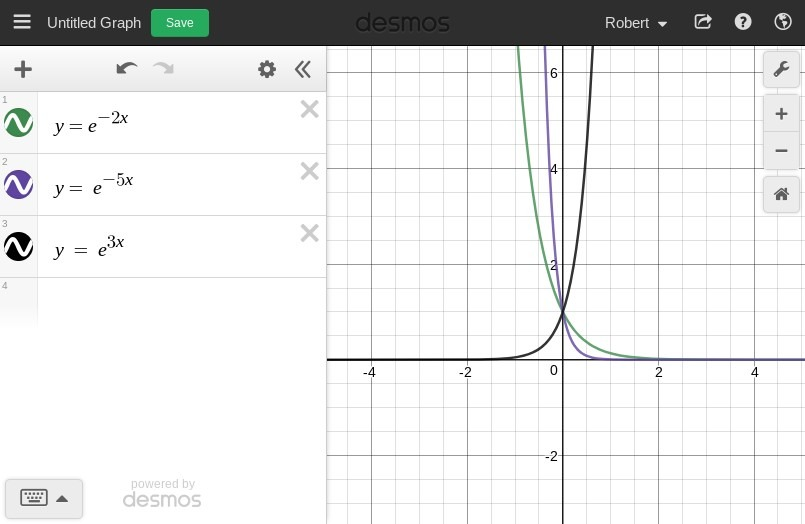
\includegraphics[width=4in]{lab6-img1.jpeg}}
\end{center}
(Original graph on Desmos here: \url{https://www.desmos.com/calculator/azbpenr5ml}) Note that it appears that when $A$ is negative, the family members are decreasing; and when $A$ is positive, the family members are increasing. 

To see this even more interactively, you can create a family of functions in Desmos by leaving the parameter value in place and creating a slider for it. Here's the slider version of this family: \url{https://www.desmos.com/calculator/4kkywkug7h} Click on the link and play with the slider, and you can see how the parameter value changes the way the function behaves. 

This is actually exactly what you did in Lab 5, when trying to fit a logarithmic function to some data from the CDC. You created a \emph{three}-parameter family: 
$$y = a \ln(bx) + c$$
with parameters $a,b$, and $c$ and used the sliders to change the parameters so that the resulting function was a good fit to the data. If you need a refresher on how to create graphs with sliders in Desmos, please refer to the instructions for Lab 5. 

What you'll be doing differently here in Lab 6 is thinking about how to use Calculus to discover exactly how the parameter values affect the behavior of the function. For example: Go back to the one-parameter family $y = e^{Ax}$. How can we be sure that the members of this family are increasing when $A > 0$ and decreasing when $A < 0$? Well, the derivative can tell us this. Take the first derivative, keeping in mind that $A$ is a number or constant, not a variable, using the Chain Rule: 
$$y' = e^{Ax} \cdot \frac{d}{dx}[Ax] = Ae^{Ax}$$
Now, $e^{Ax}$ is always positive. Therefore is $A$ is positive, so is $Ae^{Ax}$; that means the derivative is positive, therefore $y$ (the original function) is increasing. And if $A$ is negative, $Ae^{Ax}$ is negative and therefore $y$ (the original function) is decreasing. We can also notice that if $A \neq 0$, $A e^{Ax}$ is not zero (since $e$ to any power is nonzero) --- therefore we can conclude that $y$ has no critical numbers. 

So, we can take a family of functions and find its derivative with the parameter still in it, and draw conclusions about how the entire family behaves based on the values of the parameter. That's the main idea behind this Lab. 

\subsubsection*{Before doing the main activities:}
\begin{itemize}
    \item Re-read the text above in ``Setup and Instructions'' and ask questions about anything that isn't clear. 
    \item Read, and study the examples in \emph{Active Calculus} section 3.2. In particular, Example 3.2.2 is completely worked out. 
    \item Watch the following videos at the Math Department YouTube channel: 
    \begin{itemize}
        \item Quick Review: Families of Functions (\url{https://www.youtube.com/watch?v=NYM4k8TUoII})
        \item Quick Review: Working with Families of Functions part 1 (\url{https://www.youtube.com/watch?v=zVON9b1gwew}) 
        \item Quick Review: Working with Families of Functions part 2 (\url{https://www.youtube.com/watch?v=O2sVd_P5bWo}) 
    \end{itemize}
\end{itemize}


\subsection*{Main Activities}

\begin{enumerate}
    \item Consider the one-parameter family of functions given by $f(x) = x^3 - ax^2$ where $a > 0$.
    \begin{enumerate}
        \item Make a graph of this family on Desmos by entering it in as a single function with a parameter, and create a slider for the parameter. Change the left-hand endpoint of the slider to $0$ since we are defining this parameter only for $a > 0$. (Just click on the left endpoint and it will let you change it.) Copy and paste the link into your writeup. 
        \item Play with the slider and observe how the function changes as the parameter changes. Based on your observations, how many critical numbers will any member of the family have? Are the critical numbers always in the same place, or do their locations change as $a$ changes? (Don't just answer yes or no; give some detail about what you observe.) 
        \item Based on your Desmos slider graph, how many inflection points will any member of the family have, and do the inflection points depend on $a$ or not? (Don't just answer yes or no; give some detail about what you observe.) 
        \item Calculate $f'(x)$. The result will have the parameter $a$ in it along with the variable $x$. Use this to find all the critical numbers of $f$. At least one of these will be in terms of $a$. And you should have the same number of critical numbers as you originally predicted in part (b) above. 
        \item Calculate $f''(x)$. The result, again, should have $a$ in it. 
        \item Evaluate each critical number you found into $f''(x)$ (not $f$ or $f'$, but the second derivative). Based on the Second Derivative Test (described in your readings and video for Section 3.1), use the information to classify each critical number as a local minimum, local maximum, or neither. Show all work and explain your process. 
        \item Use $f''$ to locate the inflection point on this family, and give its $x$-coordinate in terms of the parameter $a$. 
    \end{enumerate}
    
Before submitting any work on this problem, double check your answers by making observations from your graph. For example if computed five critical numbers for $f$ but your graph only shows two of them, of if you computed the inflection points but your graph doesn't show any inflection points, rectify your graph with your calculus and algebra first before submitting your work. This will save you a revision. 

\item Pick EXACTLY ONE of the following to do as a second item on this lab. 
    \begin{enumerate}
        \item Consider the two-parameter family given by: 
        $$E(x) = e^{-\frac{(x-m)^2}{2s^2}}$$
        where $m$ is any real number and $s > 0$. Make a graph of this two-parameter family on Desmos with sliders, and copy/paste the link. This family describes the \emph{normal distribution} or ``bell curve'' very common in statistics, science, and social science. From the graph, describe how changing $m$ and $s$ affects the shape of the curve. Use Wolfram\textbar Alpha to find $E'(x)$ in terms of $x$ and the two parameters; and then show that $E$ has exactly one critical number, at $x = m$. 
        \item Consider the three-parameter family given by: 
        $$L(t) = \frac{A}{1 + ce^{-kt}}$$
        where $A,c$, and $k$ are all positive real numbers. Make a graph of this two-parameter family on Desmos with sliders, and copy/paste the link. This family describes \emph{logistic growth}, very common in population biology and psychological phenomena --- any growth that exibits fast initial growth followed by a slowdown in growth. Use the fact that 
        $$L''(t) = Ack^2e^{-kt} \frac{ce^{-kt}-1}{(1+ce^{-kt})^3}$$
        to create a sign chart for the second derivative, and then locate where the inflection point on $L$ happens (in terms of the parameters). (As always, show your work.) If $L$ represents the growth in some quantity over time, then what is the significance of the inflection point in terms of growth? 

\end{enumerate}

	
\end{document}